% !TEX root = ../rawlik-phd-thesis.tex
\chapter{Axion analysis}
\label{ch:axion-analysis}

Now that the foundation of the analysis has been explained we proceed to present how were they applied to the data. The data have been taken at PSI in the years 2015-17 during nEDM runs (as in no dedicated runs have been done.)

Explain why short and long time-base analyses. Mention the axion wind analysis already.

In this analysis two couplings were considered. The first is scalar and looks like an oscillating nEDM. The second is vector and acts like an oscillating magnetic field.

The analysis has been divided in two based also on an another criterion. The long time--base and short time--base. The first used the data set of the nEDM experiment performed in ILL by the Sussex--RAL--ILL collaboration and covers oscillation periods up to days. The short time--base analysis used the PSI data set. The latter is the subject of this work, the former is part of the doctoral thesis of Nicholas Ayres \mnote{Cite Nick's PhD here}. We have closely collaborated.



\section{How a signal would look like}
It is instructive to first understand well how would an axion signal come up in the data.

The main purpose of the experiment is to measure the static neutron electric dipole moment. This would appear as a shift in $R$\mnote{Needs to be clear that the reader is familiar with $R$ here.} dependent on direction of the electric field relative to the magnetic one. In zero electric there would be no shift, while the parallel and anti--parallel configurations of the magnetic and electric fields would shift $R$ in opposite directions. Due to the data blinding
\footnote{In order to reduce bias the data were modified upon being taken in a way, that a secret nEDM was injected into them. This additional offset is only revealed as the very last step, once the measurement and analysis have been completed. The data were still blinded at the time of writing.}
we expect a pronounce shift corresponding to an nEDM of \SI{e-25}{\elementarycharge\centi\meter}.

Should the neutron electric dipole moment oscillate, $R$ would oscillate as well, even if the electric field is kept constant. A reversal of the electric field polarity would reverse the phase of the oscillations. At zero electric field no oscillations would be visible. In Fig.\,\ref{fig:axions_data_taking_one_run} we depict an $R$ time--series with the combined effect of a large nEDM oscillation and the blinding offset.

\begin{figure}[bth]
  \myfloatalign
  \subfloat
  [An oscillating neutron electric dipole moment signal in the nEDM @ PSI apparatus. The colours indicate different electric field states: parallel to the magnetic field, antiparallel to it and zero]
  {\label{fig:axions_data_taking_one_run}
  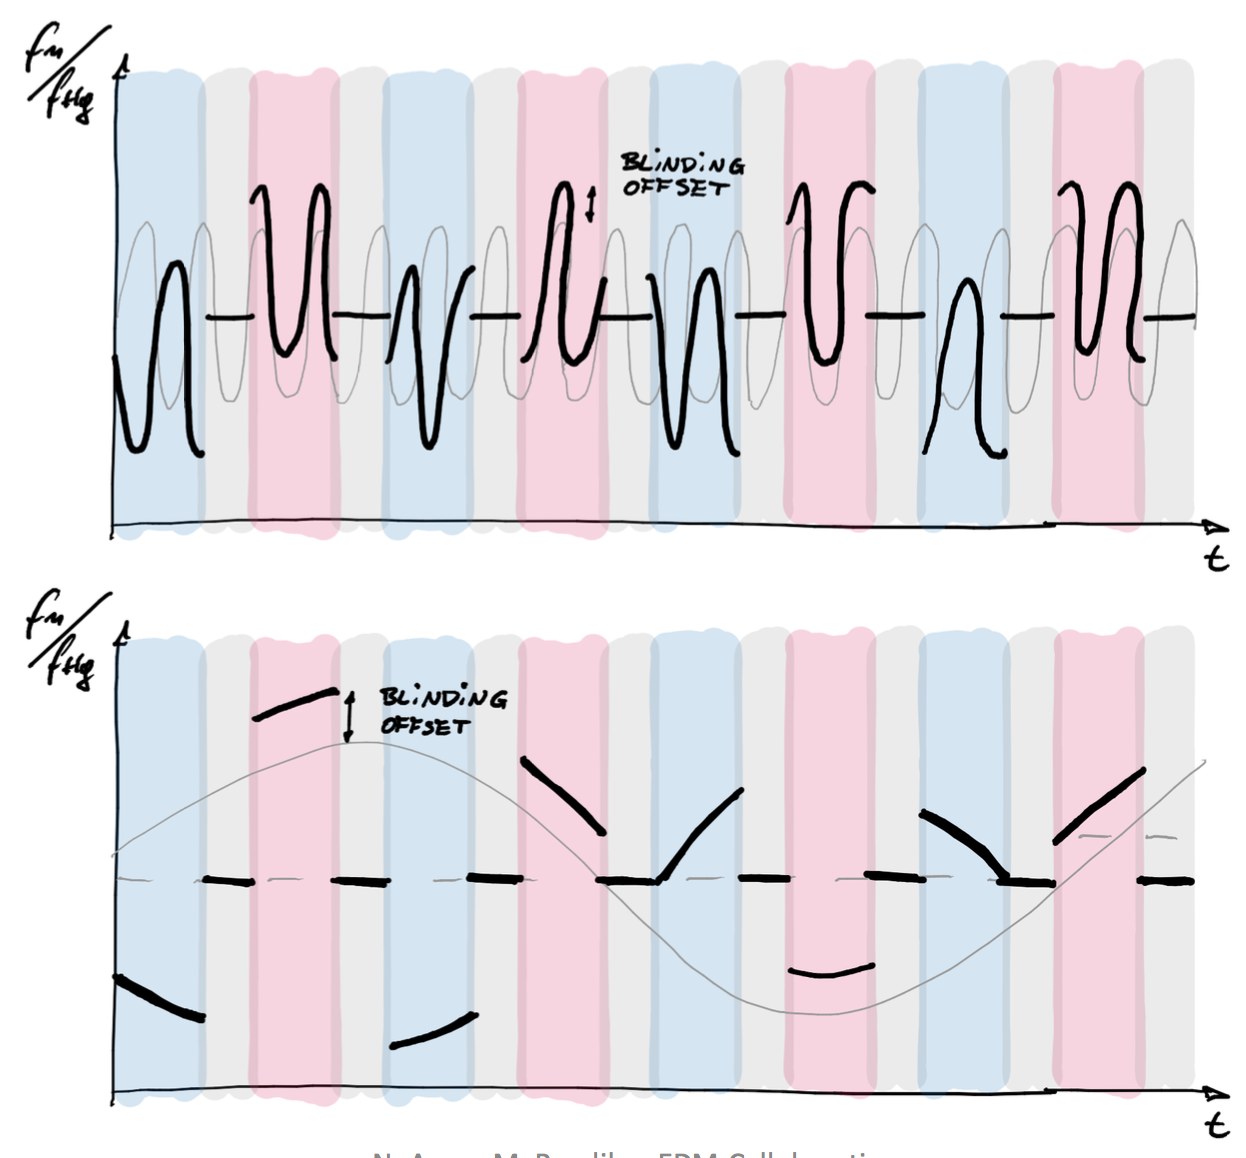
\includegraphics[width=.34\linewidth]{gfx/axions/cycle-level_blinding_offset.png}}
  \quad
  \subfloat
  [An oscillating neutron electric dipole moment signal in the nEDM @ PSI apparatus across many runs. The colours indicate different electric field states: parallel to the magnetic field, antiparallel to it and zero. Different runs have different magnetic field gradients, which causes each run to have a different shift in $R = f_n / f_{Hg}$.]
  {\label{fig:axions_data_taking_runs}
  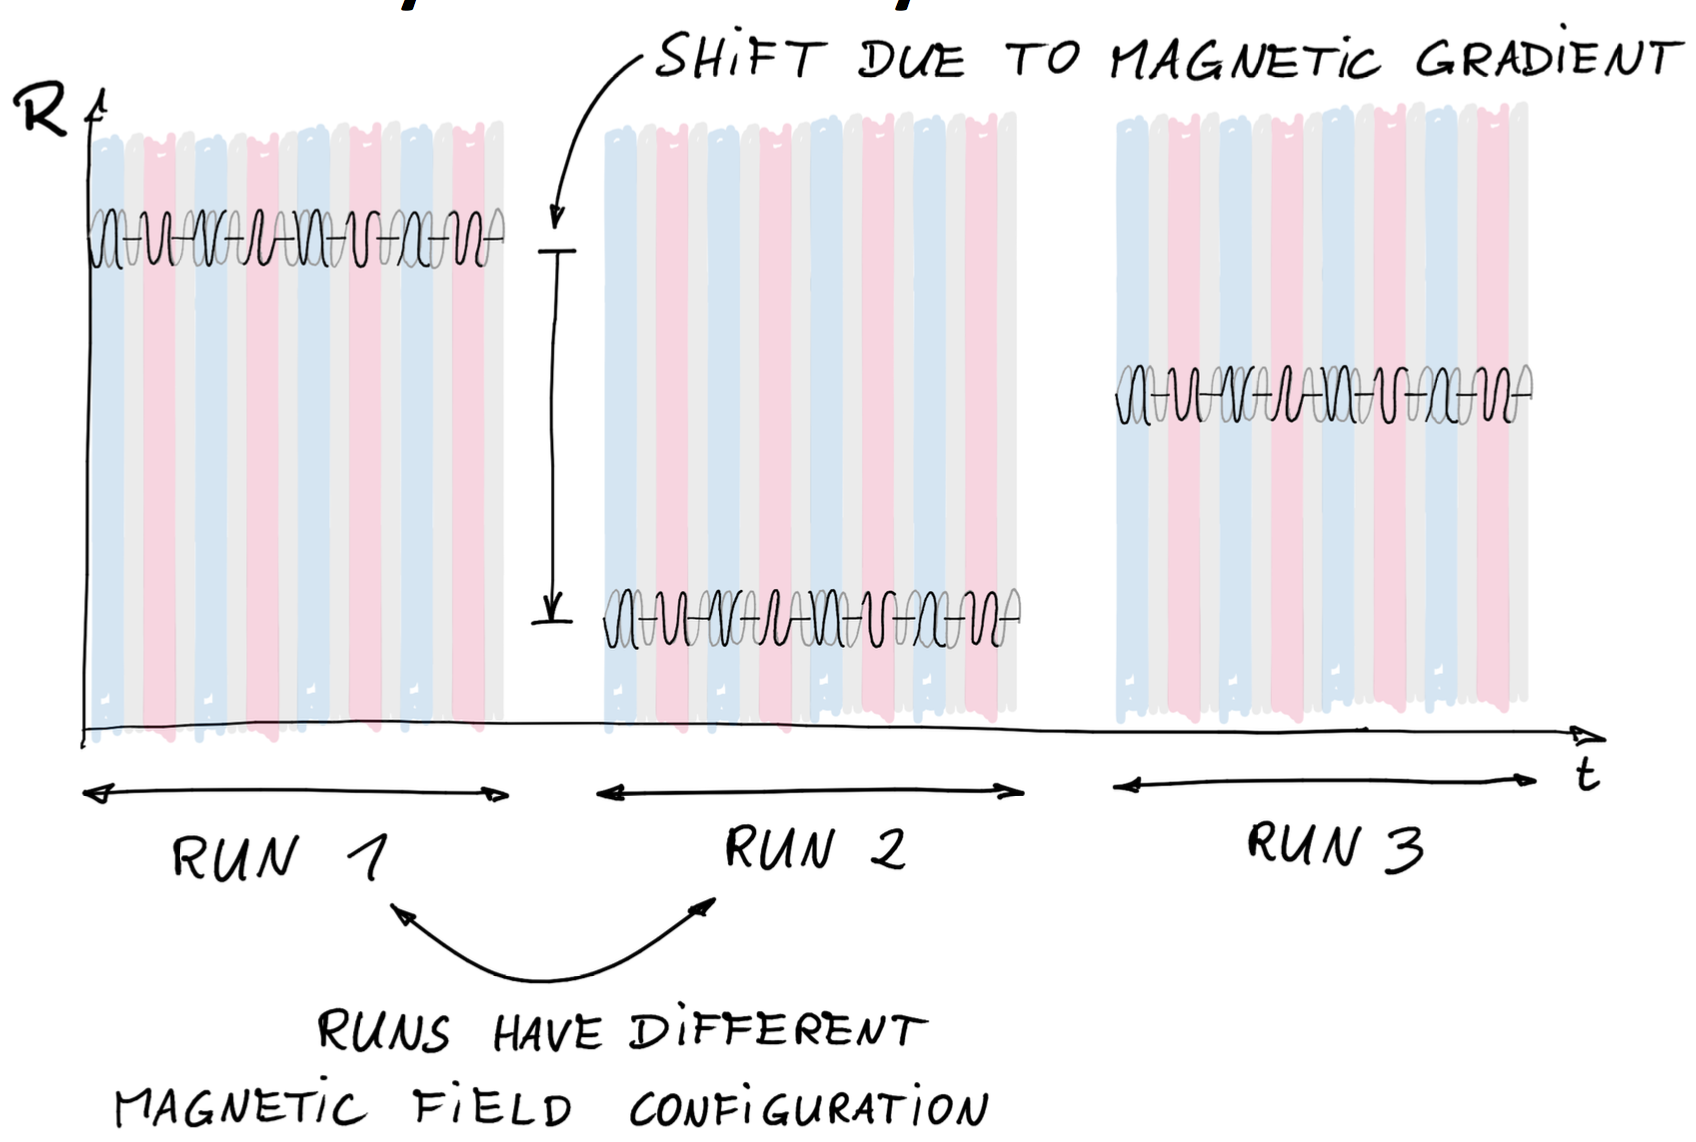
\includegraphics[width=.56\linewidth]{gfx/axions/cycle-level_gradient_jump.png}}
  \caption{The data taking scheme in the nEDM experiment at PSI.}
\end{figure}

A part of the measurement procedure is to deliberately work in a magnetic field gradient, as explained\ldots \mnote{Need to explain in somewhere, best at the beginning.} The vertical magnetic filed gradient changes substantially when a new run is started. \mnote{Give the reasons why it changes: we apply a new one, which follows from the measurement procedure} Thereby $R$ is shifted by a big value, changing the DC level of the oscillating nEDM signal, which is illustrated in Fig.\,\ref{fig:axions_data_taking_runs}. Moreover, even during a single run the gradient drifts, as clearly visible in Fig.\,\ref{fig:axions_gradient_drift_correction}. \mnote{Write here, that we can do a good relative gradient drift correction, but not an absolute one.}

\begin{figure}[bth]
  %FIXME directly copied from Elise's presentation on the 2015 PSI collaboration meeting
  \myfloatalign
  \subfloat
  [Another time series of $R$ in the nEDM experiment. The colours depict electric field states, black being no electric field. A drift is clearly visible.]
  {\label{fig:axions_gradient_drift_not_corrected}
  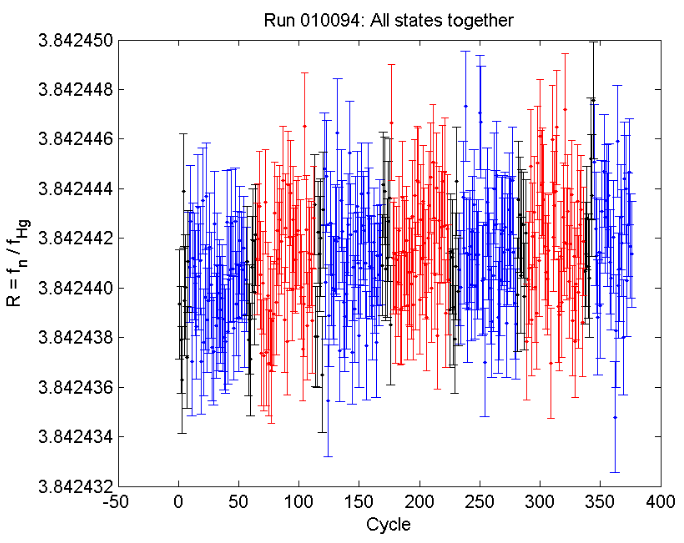
\includegraphics[width=.45\linewidth]{gfx/axions/gradient_drift_elise}}
  \quad
  \subfloat
  [The data as on Fig.\,\ref{fig:axions_gradient_drift_not_corrected} corrected for gradient fluctuations.]
  {\label{fig:axions_gradient_drift_corrected}
  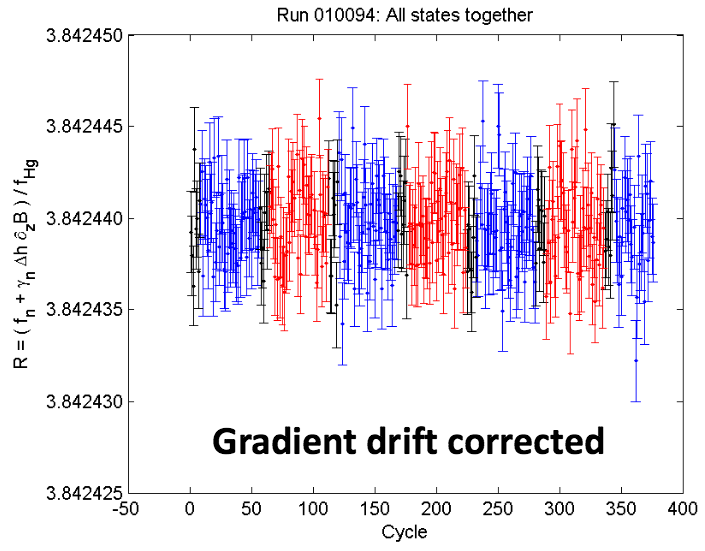
\includegraphics[width=.45\linewidth]{gfx/axions/gradient_drift_elise_corrected}}
  \caption{Correcting the $R$ time series for fluctuations of the vertical magnetic field gradient.}
  \label{fig:axions_gradient_drift_correction}
\end{figure}

The nEDM team spares no effort to measure the gradient. Nevertheless, the achieved precision (\SI[per-mode=symbol]{\approx 1}{\pico\tesla\per\centi\meter}) is only comparable to the one of $f_n$ (in the order of \SI{1}{\pico\tesla}). The exact way how the gradient should determined is highly non--trivial and there is ongoing research in this respect. \mnote{Mention here the exact way the gradient drift correction is done. And cite Elise's thesis.} Actually, even the height difference between the neturons and $^{199}$Hg centres of mass (a few milimeters) is still discussed. \mnote{Know how exactly was $\Delta h$ determined in the end. Also, mention the definition of a sequence here (as in the paper).} % Assuming a constant gradient during a \emph{run} one can determine it much more precise. This assumption, however, is known not to be exactly true.

One should note, that any, including an oscillating one, nEDM effect affects only the position of the neutrons' resonance. The shape of the resonance curve is unaffected. Therefore, the method to extract neutron Larmor frequency $f_n$, and thereby $R$, for each \emph{cycle} is valid also in case of an oscillating nEDM.

It may be tempting to think about demodulating the $R$ time--series into what would be expected to be an oscillation. This would require subtracting the DC offset for each electric field configuration, in each run separately, then flipping the signal around the DC level for one configuration. \mnote{The offsets are measured with Cs, mention that.} The disadvantage is that uncertainty in such a demodulation would become a systematic effect and would need to be tightly controlled.

A different approach, one that that was taken, is to split the $R$ time--series into three sets: without the electric field (a control data set, no signal expected), with the electric and magnetic field parallel, and with anti-parallel (the signal is expected to come up with an opposite phase in the two). Then in the LSSA fit instead of one DC offset, allow a different one for each run:
\begin{equation}
  A\sin(2 \pi f t) + B\cos(2 \pi f t) + \sum_i C_i\,\Pi_i(t) \,
\end{equation}
where $C_i$ is the free offset in the $i$th sequence and $\Pi_i(t)$ is a gate function equal to one in the $i$th sequence and zero elsewhere.
\mnote{The sensitivity deserves a separate paragraph somewhere later in the text.}






\section{Systematic Studies for the Cycle--Level Analysis}
While the run--level analysis can benefit from all of the systematic studies done for the constant nEDM measurement, this is not the case for the lower level cycle--level analysis. An important decision has to be taken on how to treat the systematic effects. There are three options:
% \begin{enumerate}
%   \item Perform a detailed study of time--dependent systematic effect.
%   \item Determine \emph{delicate} frequencies and cut them out.
%   \item Assume there are no systematic effects.
% \end{enumerate}

\paragraph{Perform a detail study of time--dependent systematic effect.}
Here we would assume that any excess in power, in any dataset ($E \uparrow \uparrow B$, $E \uparrow \downarrow B$ and $E=0$) is a signature of some kind of a signal. All effects that can potentially result in that should be identified before the analysis is performed and corrected for. This would require a long and careful systematic study, a task much bigger then this analysis itself. Moreover, the full--fledged systematic studies for the constant nEDM analysis of the PSI data are still ongoing. Even though we acknowledge that this would be \emph{the} proper way to go, we consider it to be unrealistic and unnecessary for this analysis.

\paragraph{Determine \emph{delicate} frequencies and cut them out.}
Looking at periodograms of raw data one sees that there are several typical frequencies where peaks appear. Typically at inverse specific time constants at which the experiment operates: cycle separation, day, week, , HV--reversal, B0--reversal. We may decide that all systematic effects are constrained to these frequencies and do not perform the analysis there at all.

\paragraph{Assume there are no systematic effects.}
An axion would produce a very specific signal, in particular:
\begin{enumerate}
  \item There would be no signal in the $E=0$ dataset.
  \item The signal would appear in both $E~\uparrow~\uparrow~B$ and $E~\uparrow~\downarrow~B$ datasets, with equal amplitude.
  \item The signals in $E \uparrow \uparrow B$ and $E \uparrow \downarrow B$ would be shifted in phase by 180~degrees.
  \item The signals would have to have a high coherence of $\delta f / f = 10^{-6}$.
\end{enumerate}
In case we see an excess in power, we would only call it a candidate for an axion--signal if the three above conditions are met. Otherwise we attribute it to a, potentially unknown, systematic effect. We do realise the danger of making the systematic search dependent of the act of finding a signal. This automatically opens a line of attack on this analysis: we would not make a discovery, because a systematic effect has canceled the real signal out. We would not have seen a signal and therefore not looked for systematic effects. This is certainly valid. Nevertheless, we argue that the extremely low probability of this event, due to the high coherence of the axion field, makes it negligible. In order to cancel the axion signal, a systematic effect would not only need to be as coherent as the axion field, but additionally fine--tuned over at least 5 orders of magnitude magnitude of tested frequencies. With the coherence of $\delta f / f = 10^{-6}$ this is a tuning of $10^{-30}$. It would also need to be fine--tuned in amplitude over $\sim 20$ orders of magnitude, which gives a rough estimate of the cancellation probability: $10^{-50}$. As we are presenting limits with 95\% C.L., we feel this approach is justified.

Out of the three, we opt for the third option, but leave the subject open to discussion for the collaboration.









\section{The analysis itself}
The PSI data set is taken 2015-07-03, 14:21:30 to 2016-12-18, 19:51:23

Definitely put in the plots for all three analyses (E0, EBp and EBap)!

This does not need to be explained really in detail! Most of the things were already explained earlier...

The largest missing piece is the Cs gradient-drift correction. What should I do with it?

First, present the results of the analysis itself. Present the periodogram, and so on...
s
Really, really first, show some example runs. Fig.\,\ref{fig:PSI_dataset_time_domain}.

\begin{figure}
  \centering
  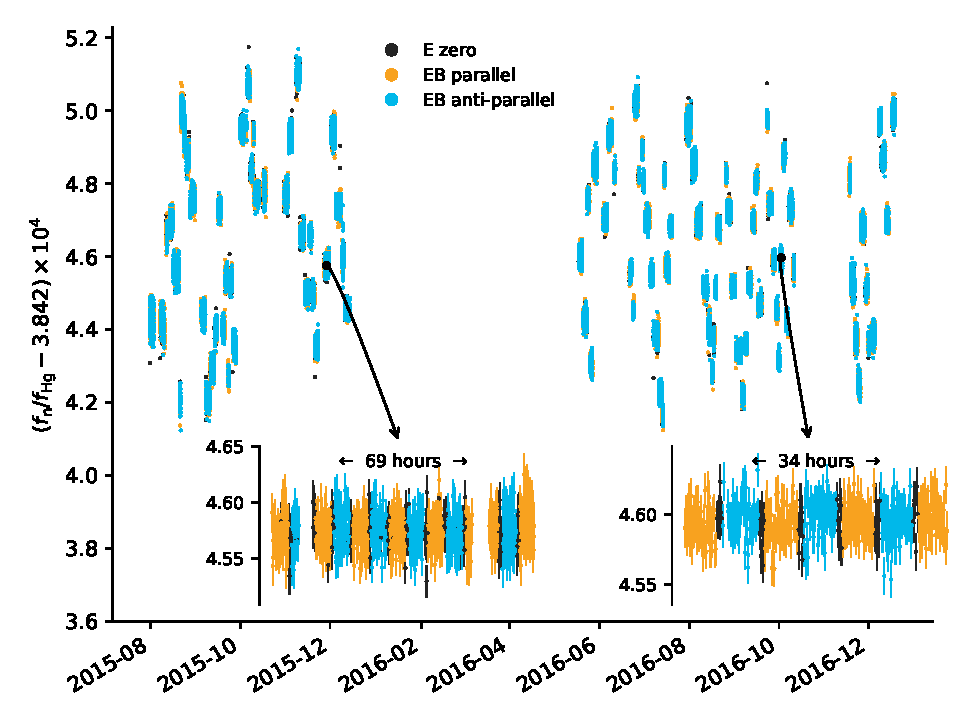
\includegraphics[width=\linewidth]{gfx/axions/deltah4mm_time_domain_inset_no_yerr.pdf}
  \caption{The complete PSI data set used in the analysis. It spans from July 2015 to December 2016. Two sequences are enlarged. The $R$ time series has been corrected for gradient drifts.}
  \label{fig:PSI_dataset_time_domain}
\end{figure}

Then proceed to discuss the results. Probably need to explain that more in detail.

\begin{figure}
  \centering
  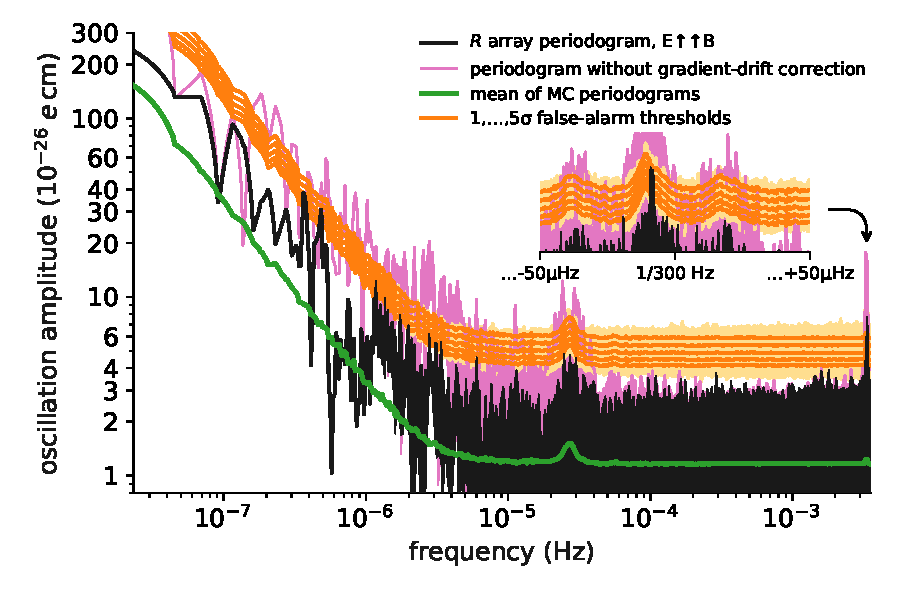
\includegraphics[width=\linewidth]{gfx/axions/detection_psi_inset_gc.pdf}
  \caption{Periodogram of the $R$ time array of the PSI experiment data, sensitive to oscillations in the quantity $d_\mathrm{n} - \left( \mu_\mathrm{n} / \mu_\mathrm{Hg} \right) \, d_\mathrm{Hg}$, taken with the $\boldsymbol{E}$ and $\boldsymbol{B}$ fields parallel (black line).
  The mean of MC--generated periodograms, assuming no signal, is depicted in green. MC is used to calculate $1,2,…,5\,\sigma$ false--alarm thresholds, depicted in light orange.
  For clarity, we also plot the smoothed version in orange.
  There are two regions where a rise in the amplitude is expected, namely around \SI{28}{\micro\hertz} (inverse of 10 hours) and \SI{3.3}{\milli\hertz} (inverse of 300 seconds), due to the time structure of the data taking (see the main text for more details). The periodogram of non-gradient-drift-corrected data is shown in pink.}
  \label{fig:axions_PSI_detection}
\end{figure}

Here would be a place to discuss the look-elsewhere effect -- how the false-alarm thresholds were obtained. Put in the plots for all three analyses! Worst case I have a lot of pages with Figures only.

\begin{figure}
  \centering
  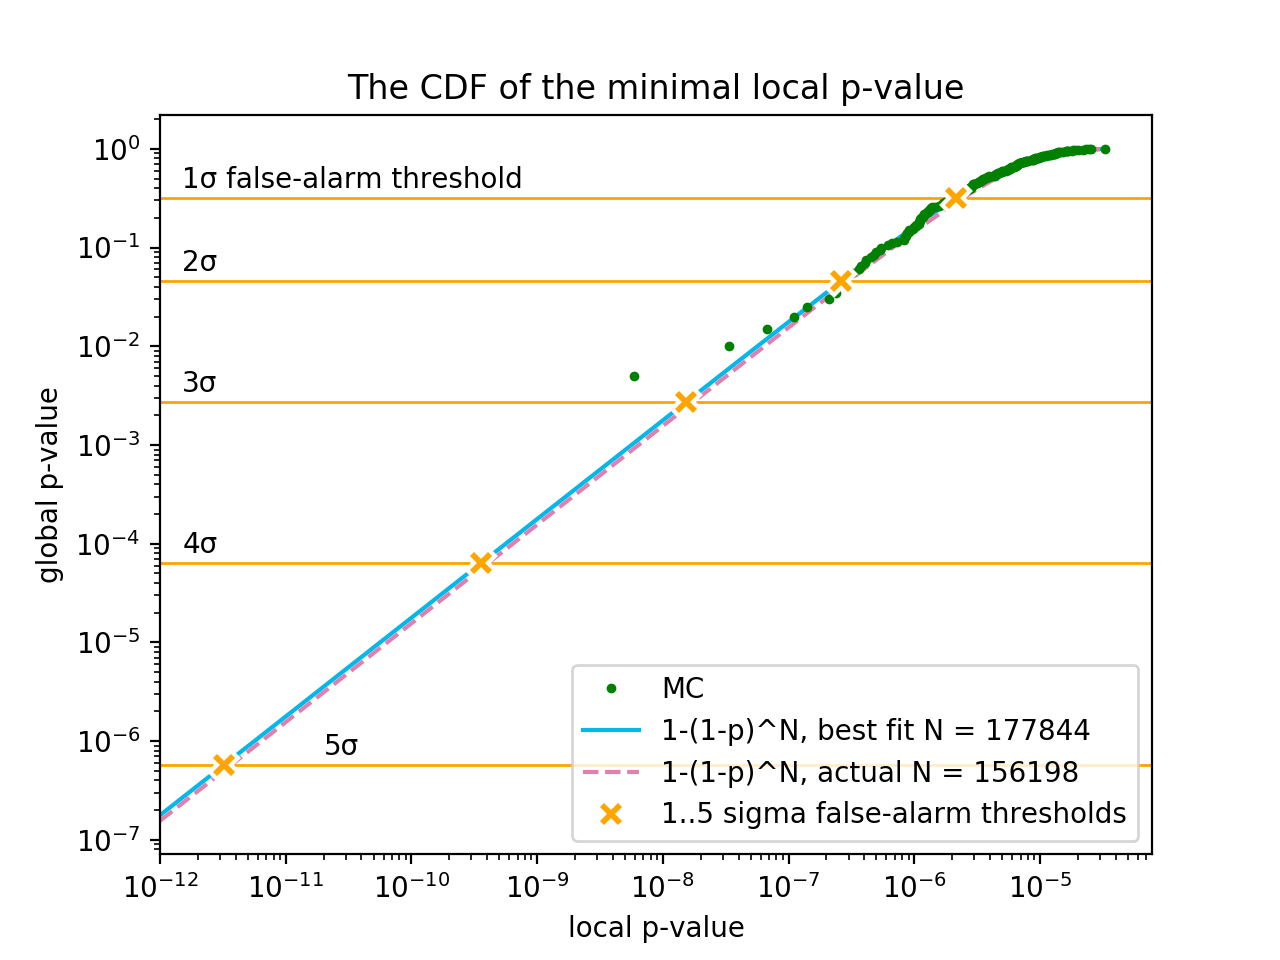
\includegraphics[width=\linewidth]{gfx/axions/P_look-elsewhere.png}
  \caption{Accounting for the look-elsewhere effect for the parallel dataset. It provides the minimal local p-value -- global p-value transition. The fit with the model \dots gives the number of frequencies.}
  \label{fig:P_look-elsewhere}
\end{figure}



\section{Discussion of the results}

There are two regions of expected rise in the oscillation amplitude due to the time structure of the data collection.
The one around $\unit[28]{\upmu Hz}$ (the inverse of 10 hours) corresponds to the period of the electric-field reversal.
The very narrow one around $\unit[3.3]{mHz}$ (the inverse of $\unit[300]{s}$) corresponds to the cycle repetition rate.
There are five
%\note{NA does anybody know what style guide says about when numbers should be written in words i.e. seven vs 7? I personally think small numbers without units should be words but this comes down to preference} ***I THINK LESS THAN TEN IT IS IN WORDS - MALCOLM ***
trial frequencies for which the $3\sigma$ false--alarm threshold is exceeded,
%\note{PMM: use words like 'surpassed', or 'exceeded' instead of penetrated}
two of which, including the largest excess with a $6\sigma$ significance, occur in a $\unit[100]{\upmu Hz}$ region around the inverse of \unit[300]{s}, while the other three are in the low-frequency region (inverse days) already excluded by the long time--base analysis.
% \note{FP: Can you maybe also explicitly state the positions of these three lines in Hz or inverse time?}
 The periodograms for the other two datasets (not shown) are very similar.
In the other sensitive set, there are three excesses of the $3\sigma$ threshold (the highest is $5\sigma$), all constrained to the same two regions. In the control dataset, only the $1\sigma$ threshold is exceeded.
%\note{MR: We may consider not discussing the false--alarm threshold penetrations, and just state in the next paragraph that we do not find a signal which meets our criteria.}
The periodogram of the $R$ time array without the gradient-drift correction is shown in pink in Fig.\,\ref{fig:PSI_detection} to visualize the frequencies where the correction has an effect.

In the introduction, mention what would be the detection criteria.
Here, first discuss the plots.
\mnote{Need to decide, whether present the plots for all E0, EB parallel and anti-parallel, or just for one.}

Start by saying that the first 

Maybe now show more in detail the plot Fig.\,\ref{fig:P_best_signal_candidate}. This I can do just for one peak.
\begin{figure}
  \centering
  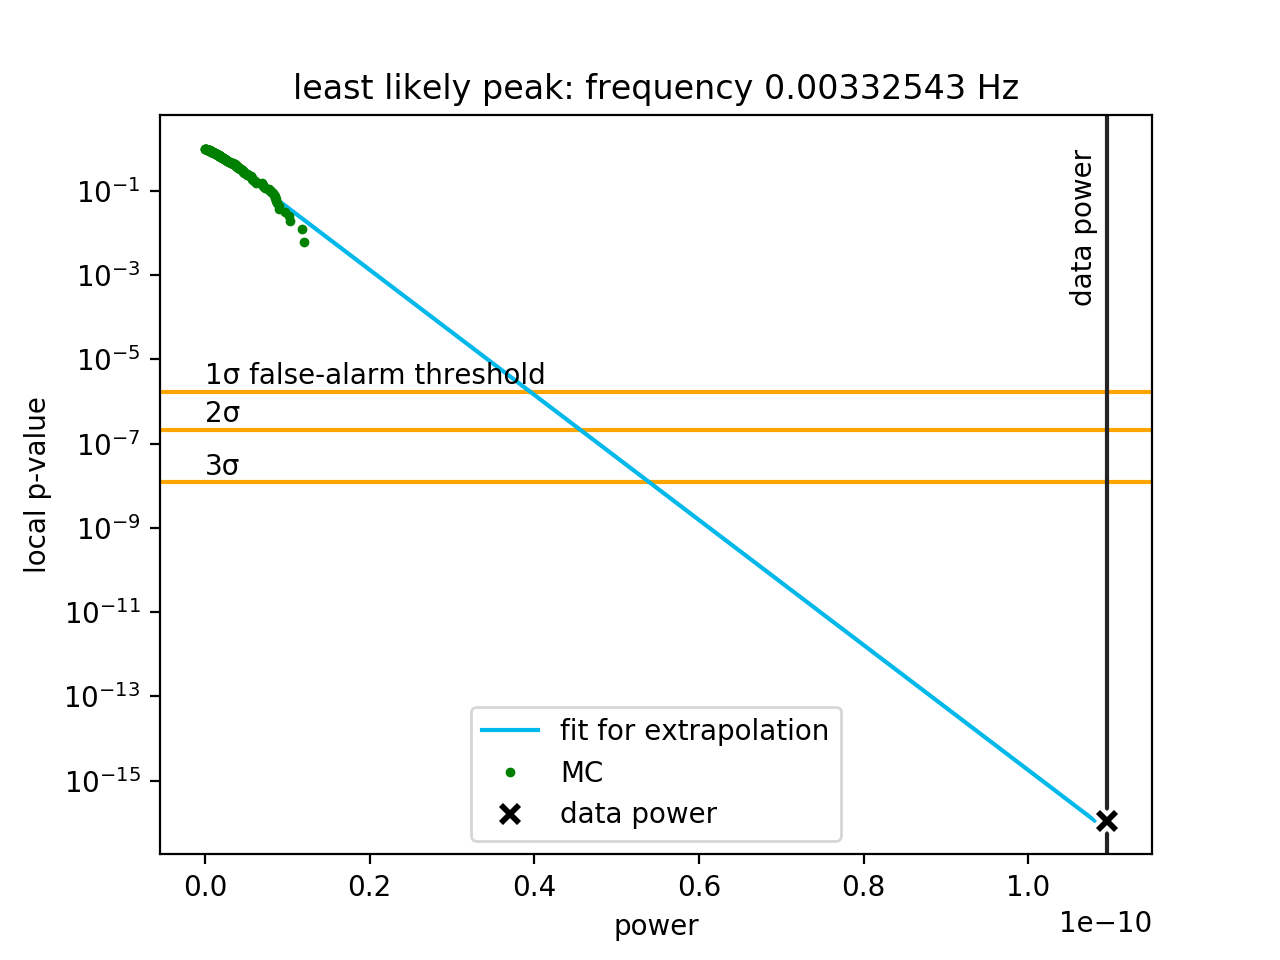
\includegraphics[width=\linewidth]{gfx/axions/P_best_signal_candidate.png}
  \caption{1 - CDF for the parallel data set. This provides the power to local p-value transition, for each frequency separately. The extrapolation based on Eq.\ldots is shown.}
  \label{fig:P_best_signal_candidate}
\end{figure}

I would list here the peaks in detail, why not? Just show the plots.


% LIST OF PEAK PLOTS




Now, proceed to discuss the distribution of p-values.
\begin{figure}
  \centering
  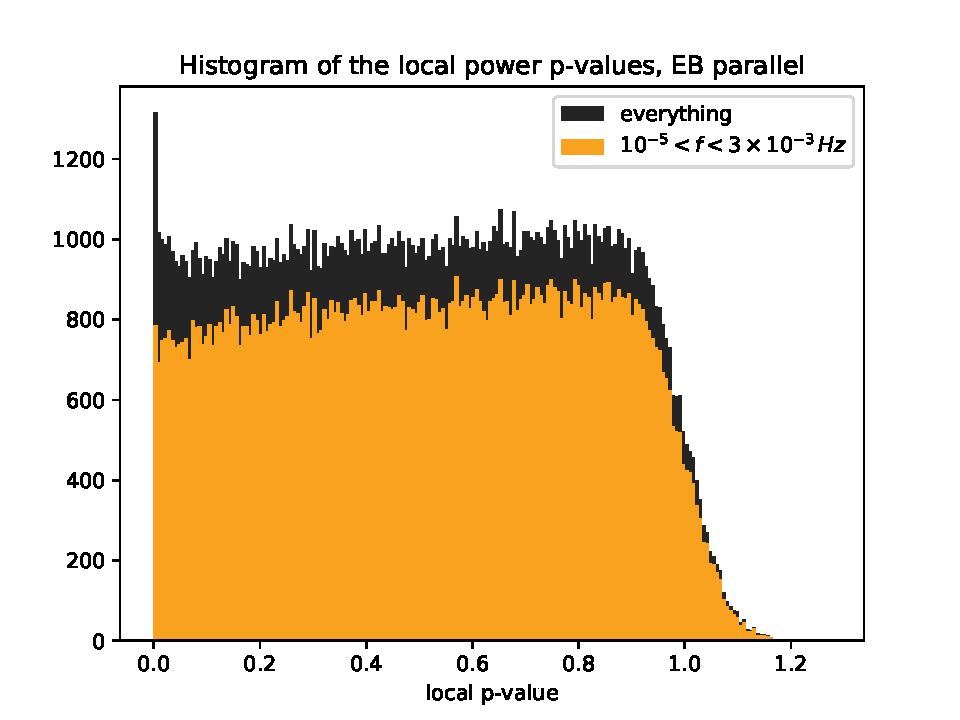
\includegraphics[width=\linewidth]{gfx/axions/P_p-values.pdf}
  \caption{Accounting for the look-elsewhere effect for the parallel dataset. It provides the minimal local p-value -- global p-value transition. The fit with the model \dots gives the number of frequencies.}
  \label{fig:P_p-values}
\end{figure}


Then, proceed to plot the filtered p-values as the function of frequency.

% HERE, a plot with the filtered p-value as the function...

\section{Axion-Wind analysis}

\section{Comparison of the analyses}
